\documentclass[12pt,a4paper,portrait]{article}
%\setcounter{secnumdepth}{0}
\usepackage{gensymb}
\usepackage{pdflscape}
\usepackage{amsmath}
\usepackage{amssymb}
\usepackage{enumitem}
\usepackage{graphicx}
\usepackage{subcaption}
\usepackage{multirow}
\usepackage{sansmath}
\setcounter{secnumdepth}{4}
\renewcommand\paragraph{\@startsection{paragraph}{4}{\z@}%
	% display heading, like subsubsection
	{-3.25ex\@plus -1ex \@minus -.2ex}%
	{1.5ex \@plus .2ex}%
	{\normalfont\normalsize\bfseries}\\}
\usepackage{pst-eucl}
\usepackage{multicol}
\usepackage{csquotes}
% Coding
\usepackage{listings}
\setlength{\parindent}{0pt}
\usepackage[obeyspaces]{url}
% Better inline directory listings
\usepackage{xcolor}
\definecolor{light-gray}{gray}{0.95}
\newcommand{\code}[1]{\colorbox{light-gray}{\texttt{#1}}}
\usepackage{adjustbox}
\usepackage[UKenglish]{isodate}
\usepackage[UKenglish]{babel}
\usepackage{float}
\usepackage[T1]{fontenc}
\usepackage{setspace}
\usepackage{sectsty}
\usepackage{longtable}
\newenvironment{tightcenter}{%
	\setlength\topsep{0pt}
	\setlength\parskip{0pt}
	\begin{center}
	}{%
	\end{center}
}
\captionsetup{width=\textwidth}
\usepackage{mbenotes} % to print table notes!
\usepackage{alphalph} % For extended counters!
% usage: \tabnotemark[3]\cmsp\tabnotemark[4]
\usepackage[colorlinks=true,linkcolor=blue,urlcolor=black,bookmarksopen=true]{hyperref}
\sectionfont{%			            % Change font of \section command
	\usefont{OT1}{phv}{b}{n}%		% bch-b-n: CharterBT-Bold font
	\sectionrule{0pt}{0pt}{-5pt}{3pt}}
\subsectionfont{
	\usefont{OT1}{phv}{b}{n}}
\newcommand{\MyName}[1]{ % Name
	\usefont{OT1}{phv}{b}{n} \begin{center}of {\LARGE  #1}\end{center}
	\par \normalsize \normalfont}
\makeatletter
\newcommand\FirstWord[1]{\@firstword#1 \@nil}%
\newcommand\@firstword{}%
\newcommand\@removecomma{}%
\def\@firstword#1 #2\@nil{\@removecomma#1,\@nil}%
\def\@removecomma#1,#2\@nil{#1}
\makeatother

\newcommand{\MyTitle}[1]{ % Name
	\Huge \usefont{OT1}{phv}{b}{n} \begin{center}#1\end{center}
	\par \normalsize \normalfont}
\newcommand{\NewPart}[1]{\section*{\uppercase{#1}}}
\newcommand{\NewSubPart}[1]{\subsection*{\hspace{0.2cm}#1}}
\renewcommand{\baselinestretch}{1.05}
\usepackage[margin=0.2cm]{geometry}
\date{}
\setcounter{tocdepth}{4}

\title{Double pendulum with first pendulum rigid and second elastic}
\author{Brenton Horne}

\begin{document}
	\maketitle
	
	In this document, we analyse the double pendulum where the second pendulum is elastic. The rest length of the elastic pendulum is $l$ and its displacement from rest is $x$. Let the masses of the pendulum bobs be $m_1$ and $m_2$, respectively. We will assume the rod/string have no mass. I have tried accounting for it, using a centre of mass approach, in my double pendulum calculation and my experience with simulations is that it does not really make things any more interesting and just adds complexity. 
	\begin{figure}[H]
		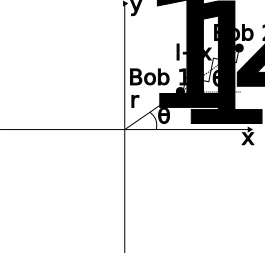
\includegraphics[width=300px]{Double pendulum second elastic.png}
	\end{figure}
	
	\tableofcontents
	
	\section{Positions and velocities}
	\begin{align*}
		x_1 &= r_1 \cos{\theta_1} &\therefore \dot{x}_1 &= -r_1 \dot{\theta}_1 \sin{\theta_1}\\
		y_1 &= r_1 \sin{\theta_1} &\therefore \dot{y}_1 &= r_1 \dot{\theta}_1 \cos{\theta_1} \\
		x_2 &= x_1 + (l+x)\cos{\theta_2} & \therefore v_1^2 &= r_1^2 \dot{\theta}_1^2\\
		&= r_1 \cos{\theta_1} + (l+x)\cos{\theta_2} &\therefore \dot{x}_2 &= -r_1 \dot{\theta}_1 \sin{\theta_1} + \dot{x} \cos{\theta_2}-(l+x)\dot{\theta}_2 \sin{\theta_2}\\
		y_2 &= y_1 + (l+x)\sin{\theta_2} \\
		&= r_1\sin{\theta_1} + (l+x)\sin{\theta_2} &\therefore \dot{y}_2 &= r_1 \dot{\theta}_1 \cos{\theta_1} + \dot{x} \sin{\theta_2}+(l+x)\dot{\theta}_2 \cos{\theta_2}
	\end{align*}
	\begin{align*}
		v_2^2 &= \left( -r_1 \dot{\theta}_1 \sin{\theta_1} + \dot{x} \cos{\theta_2}-(l+x)\dot{\theta}_2 \sin{\theta_2}\right)^2 + \left(r_1 \dot{\theta}_1 \cos{\theta_1} + \dot{x} \sin{\theta_2}+(l+x)\dot{\theta}_2 \cos{\theta_2}\right)^2 \\
		&= r_1^2 \dot{\theta}_1^2 \sin^2{\theta_1}+\dot{x}^2 \cos^2{\theta_2}+(l+x)^2 \dot{\theta}_2^2 \sin^2{\theta_2} - 2r_1 \dot{\theta}_1 \dot{x}\sin{\theta_1}\cos{\theta_2} + 2r_1 (l+x)\dot{\theta}_1 \dot{\theta}_2 \sin{\theta_1}\sin{\theta_2}\\
		&-2\dot{x}(l+x)\dot{\theta}_2 \cos{\theta_2}\sin{\theta_2}+r_1^2\dot{\theta}_1^2 \cos^2{\theta_1} + \dot{x}^2 \sin^2{\theta_2} + (l+x)^2 \dot{\theta}_2^2\cos^2{\theta_2} + 2r_1(l+x)\dot{\theta}_1\dot{\theta}_2\cos{\theta_1}\cos{\theta_2}\\
		&+2r_1\dot{x}\dot{\theta}_1 \cos{\theta_1}\sin{\theta_2}+2\dot{x}\dot{\theta}_2(l+x)\sin{\theta_2}\cos{\theta_2} \\
		&= r_1^2 \dot{\theta}_1^2 + \dot{x}^2 + (l+x)^2\dot{\theta}_2^2 + 2r_1\dot{\theta}_1 \dot{x} (\cos{\theta_1}\sin{\theta_2} - \sin{\theta_1}\cos{\theta_2}) + 2r_1(l+x)\dot{\theta}_1\dot{\theta}_2(\sin{\theta_1}\sin{\theta_2} + \cos{\theta_1}\cos{\theta_2})\\
		&+2\dot{x}\dot{\theta}_2(l+x)(\sin{\theta_2}\cos{\theta_2}-\sin{\theta_2}\cos{\theta_2})
	\end{align*}
	\begin{align*}
		v_2^2 &= r_1^2 \dot{\theta}_1^2 + \dot{x}^2 + (l+x)^2\dot{\theta}_2^2 + 2r_1\dot{\theta}_1 \dot{x} \sin{(\theta_2-\theta_1)} + 2r_1(l+x)\dot{\theta}_1\dot{\theta}_2\cos{(\theta_2 - \theta_1)}.
	\end{align*}
	\section{Generalized basis vectors}
	\begin{align*}
		\dfrac{\partial \vec{r}_1}{\partial \theta_1} &= r_1\begin{bmatrix}
			-\sin{\theta_1} \\
			\cos{\theta_1}
		\end{bmatrix} & \dfrac{\partial \vec{r}_1}{\partial \theta_2} &= \dfrac{\partial \vec{r}_1}{\partial x} \\
		\dfrac{\partial \vec{r}_2}{\partial \theta_1} &= r_1\begin{bmatrix}
			-\sin{\theta_1} \\
			\cos{\theta_1}
		\end{bmatrix} & &= 0. \\
		\dfrac{\partial \vec{r}_2}{\partial \theta_2} &= (l+x)\begin{bmatrix}
			-\sin{\theta_2} \\
			\cos{\theta_2}
		\end{bmatrix} & \dfrac{\partial \vec{r}_2}{\partial x} &= \begin{bmatrix}
		\cos{\theta_2}\\
		\sin{\theta_2}
		\end{bmatrix}.
	\end{align*}
	
	\section{Kinetic energy}
	\begin{align*}
		T &= \dfrac{m_1}{2}v_1^2 + \dfrac{m_2}{2}v_2^2 \\
		&= \dfrac{m_1r_1^2 \dot{\theta}_1^2}{2} + \dfrac{m_2(r_1^2 \dot{\theta}_1^2 + \dot{x}^2 + (l+x)^2\dot{\theta}_2^2 + 2r_1\dot{\theta}_1 \dot{x} \sin{(\theta_2-\theta_1)} + 2r_1(l+x)\dot{\theta}_1\dot{\theta}_2\cos{(\theta_2 - \theta_1)})}{2}\\
		&= \dfrac{m_1+m_2}{2}r_1^2\dot{\theta}_1^2 + \dfrac{m_2(\dot{x}^2 + (l+x)^2\dot{\theta}_2^2 + 2r_1\dot{\theta}_1[ \dot{x} \sin{(\theta_2-\theta_1)} + (l+x)\dot{\theta}_2\cos{(\theta_2 - \theta_1)}])}{2}.
	\end{align*}
	
	\section{Potential energy}
	\subsection{First bob}
	For the first bob, the only potential energy is gravitational. 
	\begin{align*}
		V_1 &= m_1gy_1 \\
		&= m_1 gr_1\sin{\theta_1}.
	\end{align*}
	
	\subsection{Second bob}
	For the second bob, there is the spring potential energy and the gravitational potential energy to consider:
	
	\begin{align*}
		V_2 &= m_2gy_2 + \dfrac{kx^2}{2} \\
		&= m_2 g(r_1\sin{\theta_1} + (l+x)\sin{\theta_2}) + \dfrac{kx^2}{2}.
	\end{align*}
	
	\subsection{Total}
	The total potential energy is therefore:
	
	\begin{align*}
		V &= V_1 + V_2 \\
		&= m_1 gr_1\sin{\theta_1} + m_2 g(r_1\sin{\theta_1} + (l+x)\sin{\theta_2}) + \dfrac{kx^2}{2}.
	\end{align*}
	
	\section{Lagrangian}
\end{document}